% Einstellen der Dokumentenklasse (möglich: book, report, article, dinbrief, beamer, scrbook, scrreprt, scrartcl)
% Einstellen der Dokumentoptionen (möglich: 11pt, twocolumn, oneside, titlepage, landscape, a4paper)
\documentclass[12pt,a4paper]{report}

% Template einbinden. Mögliche optionen:
%		chapter, section: 							definiert die oberste Gliederungsebene (default = chapter)
% 	header-line, no-header-line: 		Ein- bzw. Ausschalten der Kopfzeilentrennlinie (default = header-line)
% 	footer-line, no-footer-line: 		Ein- bzw. Ausschalten der Fußzeilentrennlinie (default = footer-line)
% 	switchhf: 											tauschen der Kopf- und Fußzeile
% 	last-page: 											Ein- bzw. Ausschalten der Gesamtseitenanzeige
% 	block:													Blocksatzformatierung aktivieren
\usepackage[onehalfspacing]{setspace}
\usepackage[]{template}

\usepackage{listings}
\usepackage{color}

\definecolor{dkgreen}{rgb}{0,0.6,0}
\definecolor{gray}{rgb}{0.5,0.5,0.5}
\definecolor{mauve}{rgb}{0.58,0,0.82}

\lstset{frame=tb,
	aboveskip=3mm,
	belowskip=3mm,
	showstringspaces=false,
	columns=flexible,
    basicstyle={\small\ttfamily},
    numbers=left,
  	numberstyle=\tiny\color{gray},
  	keywordstyle=\color{blue},
	commentstyle=\color{dkgreen},
	stringstyle=\color{mauve},
	breaklines=true,
	breakatwhitespace=false,
    tabsize=3,
    captionpos=b 
}

% Dokumentinformationen einbinden
% Meta-Tags
\hypersetup{
	colorlinks,
	linkcolor={black},
	citecolor={black},
	urlcolor={black},
	pdftitle={},
	pdfsubject={},
	pdfauthor={},
	pdfkeywords={},
	pdfcreator={latexmk}
}

% Dokumentinformationen
\author{Frederick Lahde\\Lars Grahmann}
\title{x.509}
\date{\today}

% Informationen für die Kopf- und Fußzeile
\renewcommand{\subject}{x.509 Handout}
\renewcommand{\topic}{}


\begin{document}
	% Titelseite
	\maketitlenew

	% Inhaltsverzeichnis
	\tableofcontentsnew
	\newpage

	% Start here
    \chapter{Grundlagen}
\section{Symmetrische Verschlüsselung}

Symmetrische Verschlüsselung basiert darauf, dass derselbe Schlüssel zum Ver- und Entschlüsseln verwendet wird.
Dementsprechend muss dieser Schlüssel dem Client und dem Server bekannt sein (siehe Abb. ~\ref{fig:symetric-crypto}).
  \begin{figure}[!htb]
    \center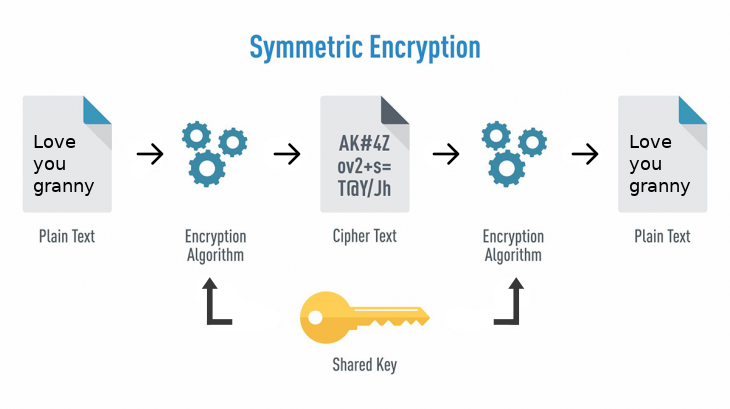
\includegraphics[scale=0.28]{images/symetric-crypto.png}
    \label{fig:symetric-crypto}
    \caption{Symmetrische Verschlüsselung}
  \end{figure}
    
\section{Asymmetrische Verschlüsselung}

Asymmetrische Verschlüsselung hingegen arbeitet auf einem öffentlichen und einem privaten Schlüssel. 
Hierbei wird der öffentliche zum Verschlüssen und der private zum Entschlüsseln verwendet.
Dadurch muss nur der private Schlüssel herausgegeben werden. (siehe Abb. ~\ref{fig:asymetric-crypto})
  \begin{figure}[!htb]
    \center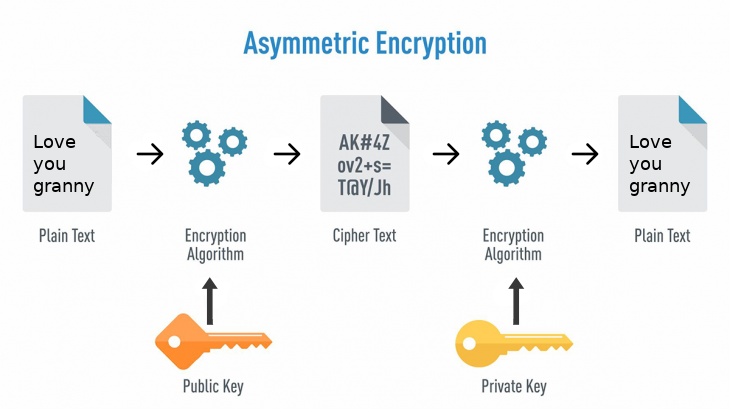
\includegraphics[scale=0.28]{images/asymetric-crypto.png}
    \caption{Asymmetrische Verschlüsselung}
    \label{fig:asymetric-crypto}
  \end{figure}

    
\section{Hash Funktionen}

Um eine große Eingabemenge auf eine kleine Zielmenge mit festgelgter Länge abzubilden, 
verwendet man sogenannte Hash Funktionen. Es gibt zahlreiche weitläufig bekannte Standards:
\begin{itemize}
    \item MD5
    \item Sha-2
    \item Argon
\end{itemize}
Eine besondere Kategorie nehmen die kryptographischen Funktionen ein: Hierbei geht es darum, eine 
Kollision zu vermeiden. Von einer Kollision wird gesprochen, wenn zwei unterschiedliche Eingabewerte zum selben Hash führen.

    
\section{Digitale Signaturen}

% TODO: Fix figure
Digitale Signature werden verwendet, um die Integrität und Authtenzität von Daten sicherzustellen. Eine Signatur ist für ein gegebenes Tupel aus
Daten und Schlüssel einzigartig. Wurde eine Nachricht entsprechend signiert, kann der Empfänger diese validieren. (siehe Abb. ~\ref{fig:signature})
\begin{figure}[!htb]
  \center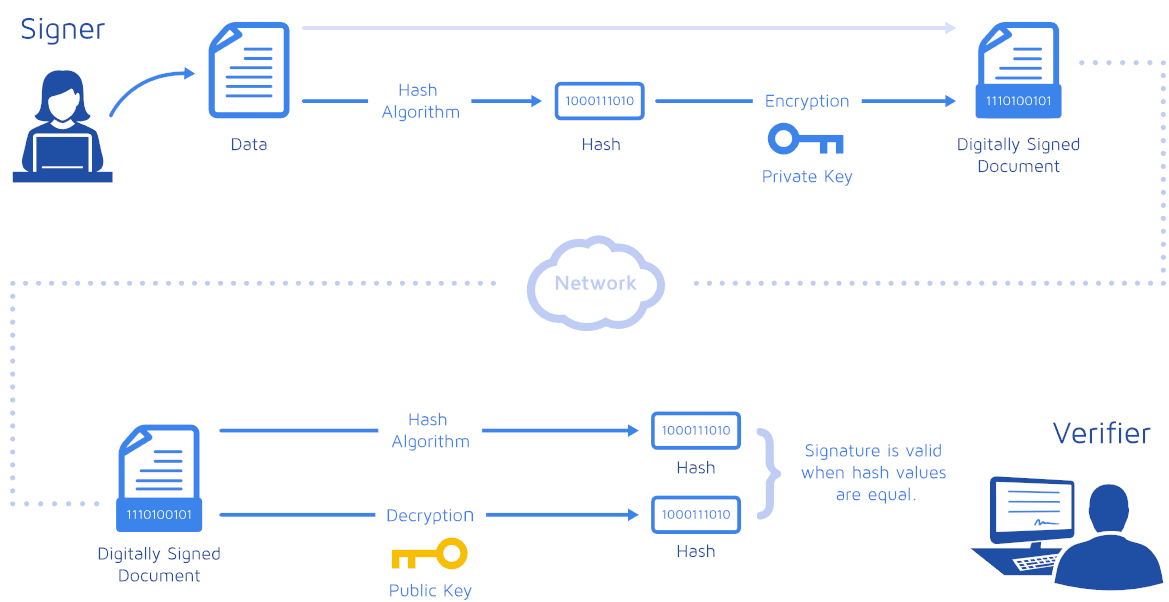
\includegraphics[scale=1.1]{images/signature-white.png}
  \label{fig:signature}
  \caption{Digitale Signatur}
\end{figure}


    \chapter{Geschichte}
X.509 wurde erstmalig am 3. Juli 1988 spezifiziert. Später wurder der Standard von der IETF\footnote{Internet Engineering Task Force} PKIX\footnote{Public-Key Infrastructure} Working Group 
weiterentwickelt und zur heutigen Form gebracht.\\
Der Standard gilt als einer der aktivsten. Während er im RFC 2459 zum ersten Mal beschrieben wurde, wurde diese Spezifikation fortlaufend überarbeitet.
So wurde dieser in den RFCs 3280 und 5280 ersetzt. Obwohl der RFC 5280 die heutige Referenz darstellt, wurde auch dieser von 6818, 8398 und 8399 geändert oder erweitert.
    

    \chapter{Zertifikate}
\section{CA}
Certificate Authorities stellen eine zentrale Stelle zum Ausgeben von Zertifkaten da. Die bekannteste dieser CA's ist Let's Encrypt~\ref{fig:lets-encrypt}, die durch das kostenlose und komplett automatisierte Austellen der Zertifikate auf viel Aufmerksamkeit von Entwicklern und Administratoren getroffen ist. 
\begin{figure}[!htb]
  \center
\includegraphics[scale=0.4]{images/lets-encrypt-transparent.png}
  \label{fig:lets-encrypt}
  \caption{Lets Encrypt}
\end{figure}

\section{CSR}
Um von einer CA ein Zertifkat zu bekommen, führt man einen sogenannten Certificate Signing Request durch. Dieser enthält Daten zur Identifiezierung des Antragstellenden, bspw. den FQDN\footnote{Fully Qualified Domain Name (git.kloud.software)} oder den Namen der Organisation. Der Anfragende erzeugt ein Schlüsselpaar und fügt den öffentlichen Schlüssel an den CSR an. Mit dem privaten Schlüssel wird der CSR signiert. Die CA prüft nun, ob die Signatur stimmt und die gelieferten Daten das ordnungsgemäße Ausstellen eines Zertifikates gemäß der Richtlinien der CA ermöglichen. Wenn alle Angaben valide sind, antwortert die CA mit einem Zertifikat welches mit ihrem privaten key signiert wurde.

\section{CRL}
In Certificate Revocation Lists werden Zertifikate aufgelistet, die von der CA vor dem Abauf ihrer Gültigkeit invalidiert wurden. Diese Invalidierung kann auf zwei Ebenen erfolgen. Einerseits kann ein Zertifkat den Status ``Hold'' zugewiesen bekommen, welches einer temporären Invaliderung entspricht, andererseits gibt es den Status ``Revoked'' welcher eine endgültige Invalidierung ausdrückt. Die Gründe dafür, dass ein Zertifkat auf einer CRL landet sind vielfältig:
\begin{itemize}
  \item unspecified (0)
  \item keyCompromise (1)
  \item CACompromise (2)
  \item affiliationChanged (3)
  \item superseded (4)
  \item cessationOfOperation (5)
  \item certificateHold (6)
  \item removeFromCRL (8)
  \item privilegeWithdrawn (9)
  \item AACompromise (10)
\end{itemize}
Wichtig zu beachten ist, dass das Konzept von CRL's nicht das Ablaufdatum der Zertifkate ersetzt. Ist ein Zertifkat abgelaufen, ist es immer als invalid zu betrachten. CRLs stellen jediglich ein weiteres Sicherheitsmerkmal von PKI da.

    \chapter{Struktur und Erweiterungen}
\section{Struktur}

  \begin{itemize}
      \item Version Number
      \item Serial Number
      \item Signature Algorithm ID
      \item Issuer Name
      \item Validity period
      \begin{itemize}
          \item not before
          \item not after
      \end{itemize}
      \item Subject Public Key Info
      \begin{itemize}
          \item Public Key Algorithm
          \item Subject Public Key
      \end{itemize}
      \item Public Key Algorithm
      \item Subject Public Key
      \item Issuer Unique Identifier (optional)
      \item Subject Unique Identifier (optional)
      \item Extensions (optional)
      \item Certificate Signature Algorithm
      \item Certificate Signature
  \end{itemize}


\section{Erweiterungen}

  \begin{itemize}
      \item Struktur
            \begin{itemize}
                \item OID identifiziert die Art der Erweiterung
                    \begin{itemize}
                        \item Basic Constraints: 2.5.29.19
                    \end{itemize}
                \item Critical indication
                    \begin{itemize}
                        \item Kritisch: Zertifikat muss abgelehnt werden, wenn Erweiterung nicht verarbeitbar
                        \item Nicht kritisch: Muss verarbeitet werden, wenn möglich
                    \end{itemize}
            \end{itemize}
  \end{itemize}



    \lstinputlisting[basicstyle=\small]{includes/extension}



    \begin{itemize}
        \item Basic Constraints: Gehört das Zertifikat zu einer CA?
        \item Key Usage: Operationen mit dem öffentlichen Schlüssel
        \item Extended Key Usage: Zweck des öffentlichen Schlüssels
            \begin{itemize}
                \item TLS \& SSL
                \item eMail Absichern
            \end{itemize}
    \end{itemize}


\section{Dateiendungen}

X.509 Zertifikate können viele verschiedene Dateiendungen haben, wobei
\begin{itemize}
\item .der
\item .crt
\item .cer
\item .pem
\end{itemize}

am häufigsten verwendet werden, aber auch 
\\\\
.p7b, .p7c, .p12, .pfx
\\\\
als verschlüsselte Daten Zertifikate enthalten sein können

    \chapter{Beispiele}
\section{End Entity Zertifikat}

    \lstinputlisting[firstline=0, lastline=10, breaklines=true]{includes/end-entity.pem}

    

    \lstinputlisting[firstline=11, lastline=20, breaklines=true]{includes/end-entity.pem}

    

    \lstinputlisting[firstline=21, lastline=30, breaklines=true]{includes/end-entity.pem}


\section{Intermediate Zertifikat}

    \begin{itemize}
        \item Subject = Issuer vom End Entity Zertifikat
    \end{itemize}
    \lstinputlisting[firstline=10, lastline=12, breaklines=true]{includes/intermediate.pem}

    

    \begin{itemize}
        \item Issuer = Subject vom Root Zertifikat
    \end{itemize}
    \lstinputlisting[firstline=6, lastline=8, breaklines=true]{includes/intermediate.pem}


\section{Root Zertifikat}

    \begin{itemize}
        \item Subject = Issuer vom End Entity Zertifikat
        \item Subject = Issuer
    \end{itemize}
    \lstinputlisting[firstline=6, lastline=12, breaklines=true]{includes/root.pem}


    \chapter{Ring of trust}
\section{Übersicht}

  Der Ring of Trust wird gebildet aus einer festen Reihenfolge der Zertifikate.
  Nach RFC 5280 wird diese Abfolge definiert. Grob zusammengefasst kann man sich
  die Abfolge der Zertifikate so vorstellen, dass Certificate Authority (kurz
  CA) einer der nächsten CA garantiert das sie vertrauenswürdig ist. Hierbei ist
  immer das ``Subject'' Feld des nächsten Zertifikats gleich dem Herausgeber des
  Vorherigen. So wird mithilfe des Privat keys von z.B. A das Zertifikat B
  verifiziert und B wurde mit dem Public key von Zertifikat A signiert. (siehe
  Abb. ~\ref{fig:certchain})\\

  \begin{figure}[!htb]
    \center 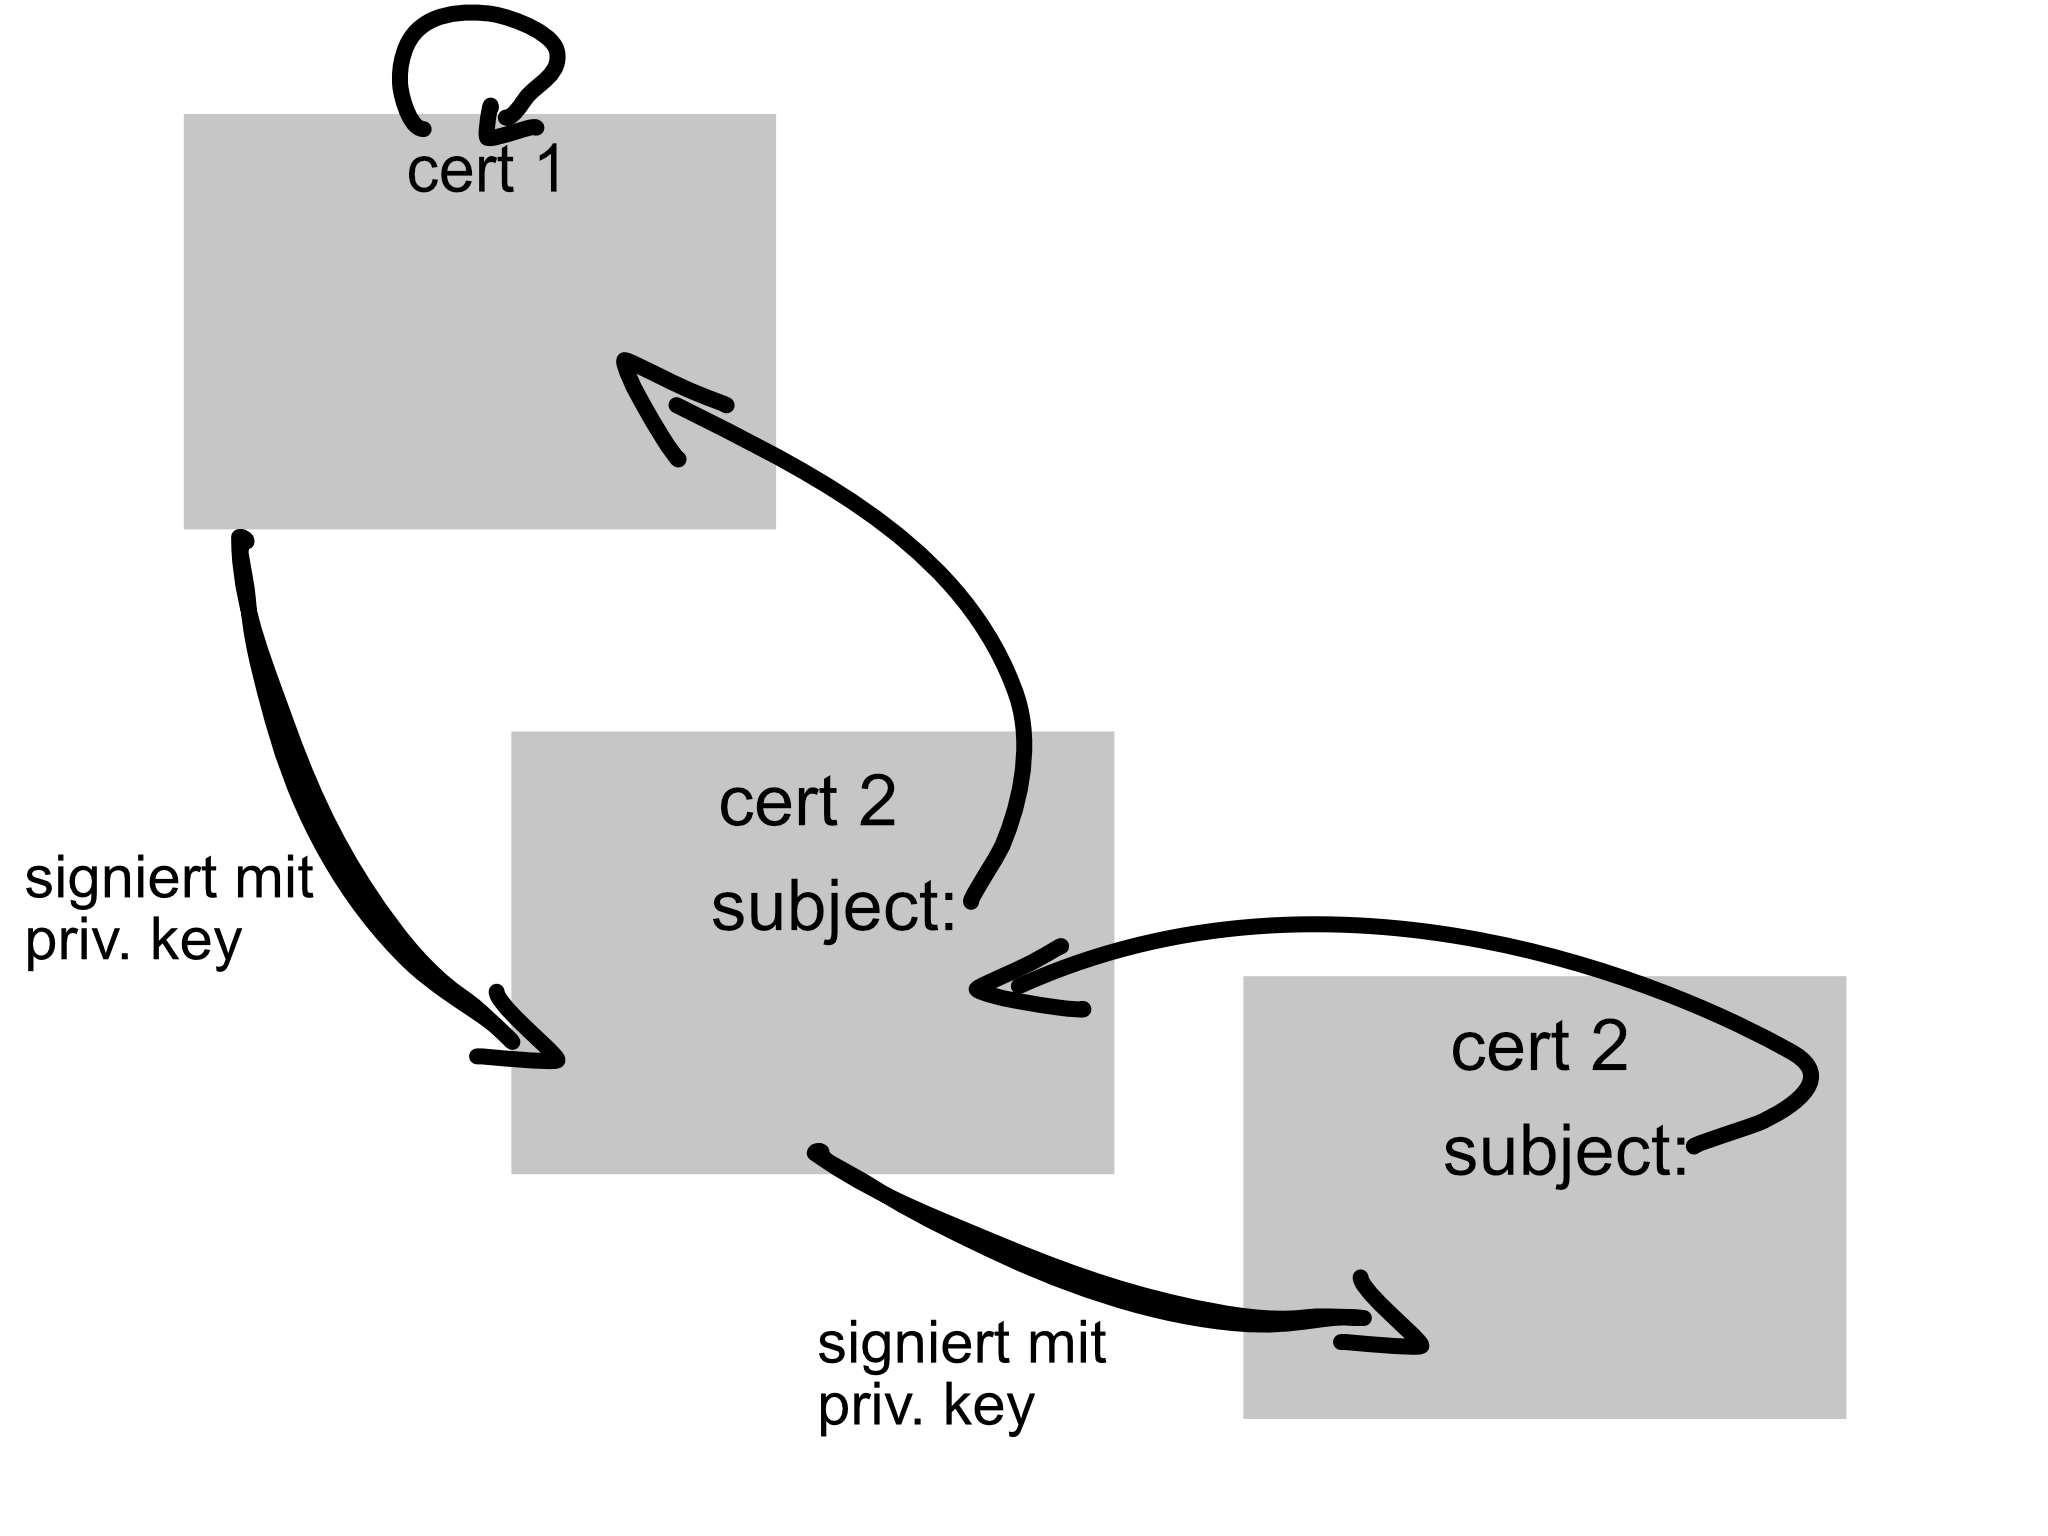
\includegraphics[scale=0.28]{images/rot.png}
    \caption{Zertifikatskette}
    \label{fig:certchain}
  \end{figure}

  \section{Root Zertifikate}
  Diese Kette löst sich so also von Zertifikat zu Zertifikat auf, bis ein s.g.
  Root Zertifikat erreicht wird. Dieses Zertifikat wurde mithilfe einer
  ``Vertrauenswürdigen Methode'' auf das Gerät übertragen. Die meisten
  Betriebsysteme haben solche Zertifikate vorinstalliert und Web-Browser haben
  auch meist eigene vertrauenswürdige Zertifikate. Diese Root Zertifikate sind
  der letzte Eintrag der Zertifikatskette und ihnen \textbf{muss} vertraut
  werden, da der Zertifikatsring hier endet.
  \pagebreak

  \section{Cross-Validierung}
  Damit CA's sich untereinander verifizieren können müssen Zertifikate kreuz
  validiert werden können. Dies wird gebraucht um zwei verschiedenen
  Verifizierungspfaden einen Weg zu schaffen Zertfikate untereinander zu
  vertrauen. Wie in Abb. ~\ref{fig:crossver} zu erkennen ist, wird für
  Kreuzvalidierung:
  \begin{enumerate}
  \item CA 1 gibt ein Zertifikat(cert 2.1) aus, was den Public key von CA 2 enthält.
  \item Nun kann mit dem nun User 2 mit seinem Zertifikat(cert 2.2) eine Vertrauenskette
    zu CA 1 über 2.1 aufbauen oder direkt zu CA 2 über cert 2
  \end{enumerate}


  \begin{figure}[!htb]
    \center 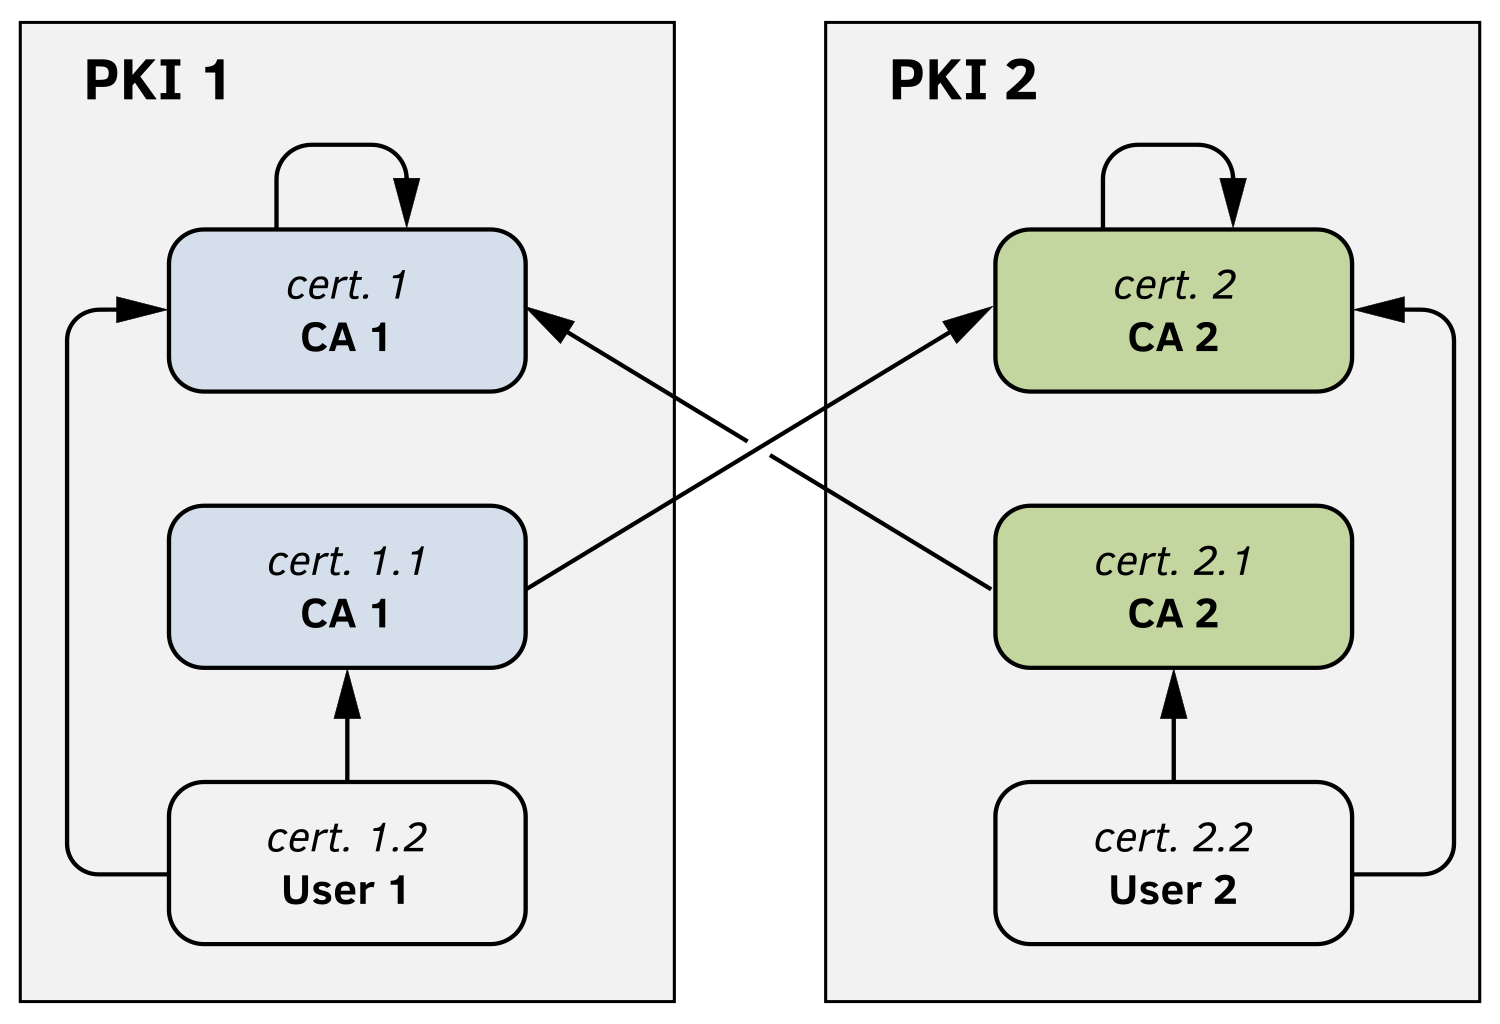
\includegraphics[scale=0.28]{images/ccd.png}
    \caption{Kreuzvalidierung}
    \label{fig:crossver}
  \end{figure}

  \section{CA Zertifikat Eneuerung}
  Um einen einfachen und leichten Übergang von auslaufenden CA Zertifikaten zu
  ermöglichen, kann die CA ein Zertifikat herausgeben, was den alten
  Public key enthält und mit dem neuen Private key signiert ist. Zeitgleich gibt
  die CA dann ein Zertifikat mit dem neuen Public key heraus, das mit dem alten
  Private key signiert ist
    \chapter{Sicherheit}
\section{Architektonische Schwächen}

  \begin{itemize}
    \item Die meisten Clients ignorieren CRL's wenn sie kein Internet haben
    \item Root Zertifikate können nicht widerrufen werden
  \end{itemize}

    

  \begin{itemize}
    \item Delegation Problem
        \begin{itemize}
            \item untergeordnete CA's können nicht vom Ausstellen von Zertifkaten außerhalb eines Namespaces abgehalten werden
            \item dadurch existieren sehr viele CA's
            \item Klassifizierung dieser nicht möglich
        \end{itemize}
  \end{itemize}

    

  \begin{itemize}
    \item Federation Problem
        \begin{itemize}
            \item untergeordnete CA's und cross signing machen Validierung komplex
            \item braucht sehr viel CPU Zeit
        \end{itemize}
  \end{itemize}

    
\section{Probleme mit CA's}

  \begin{itemize}
    \item CA's bieten so gut wie keine Gewährleistungen
    \item Expiration Date wird benutzt um den User für eine Erneuerung zur Kasse zu bitten, anstatt zur Regulierung der Stärke des Schlüssels
    \item CA's missbrauchen Sicherheitsmerkmale der Zertifikate aus ökonomischen Gründen
  \end{itemize}



  \begin{itemize}
    \item Details von CSR's sind von CA zu CA unterschiedlich, meist keine einfache Erklärung
    \item CA's sind Regierungen untergeordnet, dies widerspricht den Interessen der User
  \end{itemize}


\section{Implementations Schwächen}

  \begin{itemize}
    \item Widerrufsprüfung oft ignoriert
        \begin{itemize}
            \item werden als Hürde gesehen
            \item Infrastruktur nicht solide genug
        \end{itemize}
  \end{itemize}



  \begin{itemize}
    \item Key usage Erweiterung oft ignoriert
    \item Bestimmte Erweiterungen als kritisch zu markieren crasht clients
    \item Code Injection Attacks
  \end{itemize}


\section{Kryptographische Schwächen}

  \begin{itemize}
      \item Sicherheit von Zertifkaten baut auf Sicherheit der Hash Funktion auf
      \item Kollisionen führen zu Angriffsvektoren
      \item Angreifer können beliebige Zertifikate im Namen einer CA austellen
  \end{itemize}


    \chapter{Quellen}
\begin{itemize}
\item https://en.wikipedia.org/wiki/X.509
\item https://en.wikipedia.org/wiki/Certificate\_signing\_request
\item http://www.ietf.org/rfc/rfc1422
\item https://tools.ietf.org/html/rfc5280
\item https://tools.ietf.org/html/rfc2459
\item https://www.ietf.org/rfc/rfc3280.txt
\end{itemize}

\end{document}
